%************************************************
\chapter{Newton's Ring}
%************************************************
\begin{flushright}
August 14 and 21, 2012
\end{flushright}
\section{Aim}
	To study the fringes of equal thickness in the Newton's ring setup and hence determine the wave-length of sodium light.
\section{Apparatus}
	Sodium vapour lamp, travelling microscope, lens assembly consisting of a plane glass plate and a planoconvex lens, spherometer, magnifying glass, vernier callipers and a tiltable  glass plate assembly.

\section{Theory}
		
\section{Observations and Calculations}
	$h$ was found out to be 0.25 mm = 0.025 cm. \\
	$l$ was found out to be $\frac{4.668+3.874}{2}=4.271$ cm. (For details, refer to \autoref{1_l}) \\
	Using these, $R=\frac{l^{2}}{6h} + \frac{h}{2}$ turns out to be $121.6211$ cm.\\
	 \\
	Observations for diameter of the ring are given in \autoref{1_Diameter}.\\
	Slope of the graph of Diameter Squared, $D_{m}^{2}$ vs Order of Ring, $m$ was found to be $0.0291$ cm. (\autoref{1_graph})\\
	Using the relation
	\begin{equation}
		(D_{m})^{2}=4R\lambda m
	\end{equation}
	$\lambda=598.16\pm 3.25\%$ (where the error is calculated from the standard deviation of the slope).
	\begin{table}
		\myfloatalign
		\begin{tabularx}{\textwidth}{Xlll}
			\hline
			\tableheadline{Order of Dark Ring $m$} 	&	\tableheadline{Left (cm)} & \tableheadline{Right (cm)}\\
			\hline
				6	&	5.800	&	6.260\\
				9	&	5.755	&	6.304\\
				12	&	5.720	&	6.350\\
				13	&	5.704	&	6.360\\
				14	&	5.700	&	6.370\\
				15	&	5.670	&	6.382\\
				16	&	5.665	&	6.400\\
				19	&	5.650	&	6.420\\
				23	&	5.605	&	6.459\\
				25	&	5.600	&	6.467\\
			\hline
		\end{tabularx}
		\caption{Diameter of Newton's Ring}
		\label{1_Diameter}
	\end{table}

	\begin{table}
		\myfloatalign
		\begin{tabularx}{\textwidth}{Xlll}
			\hline
			\tableheadline{Main Scale (cm)}	& \tableheadline{Vernier Scale Division} & \tableheadline{Reading (cm)}\\
			\hline
			\tableheadline{Outer $l$}\\
				4.6	& 34 & 4.668\\
				4.6	& 35 & 4.670\\
				4.6	& 34 & 4.668\\	
			\hline
			\tableheadline{Inner $l$}\\
				3.8	& 37 & 3.874\\
				3.8	& 38 & 3.876\\
				3.8	& 37 & 3.874\\		
			\hline
		\end{tabularx}
		\caption{Measurement of $l$ of spherometer}
		\label{1_l}
	\end{table}

	\begin{figure}[bth]
		\begin{center}
			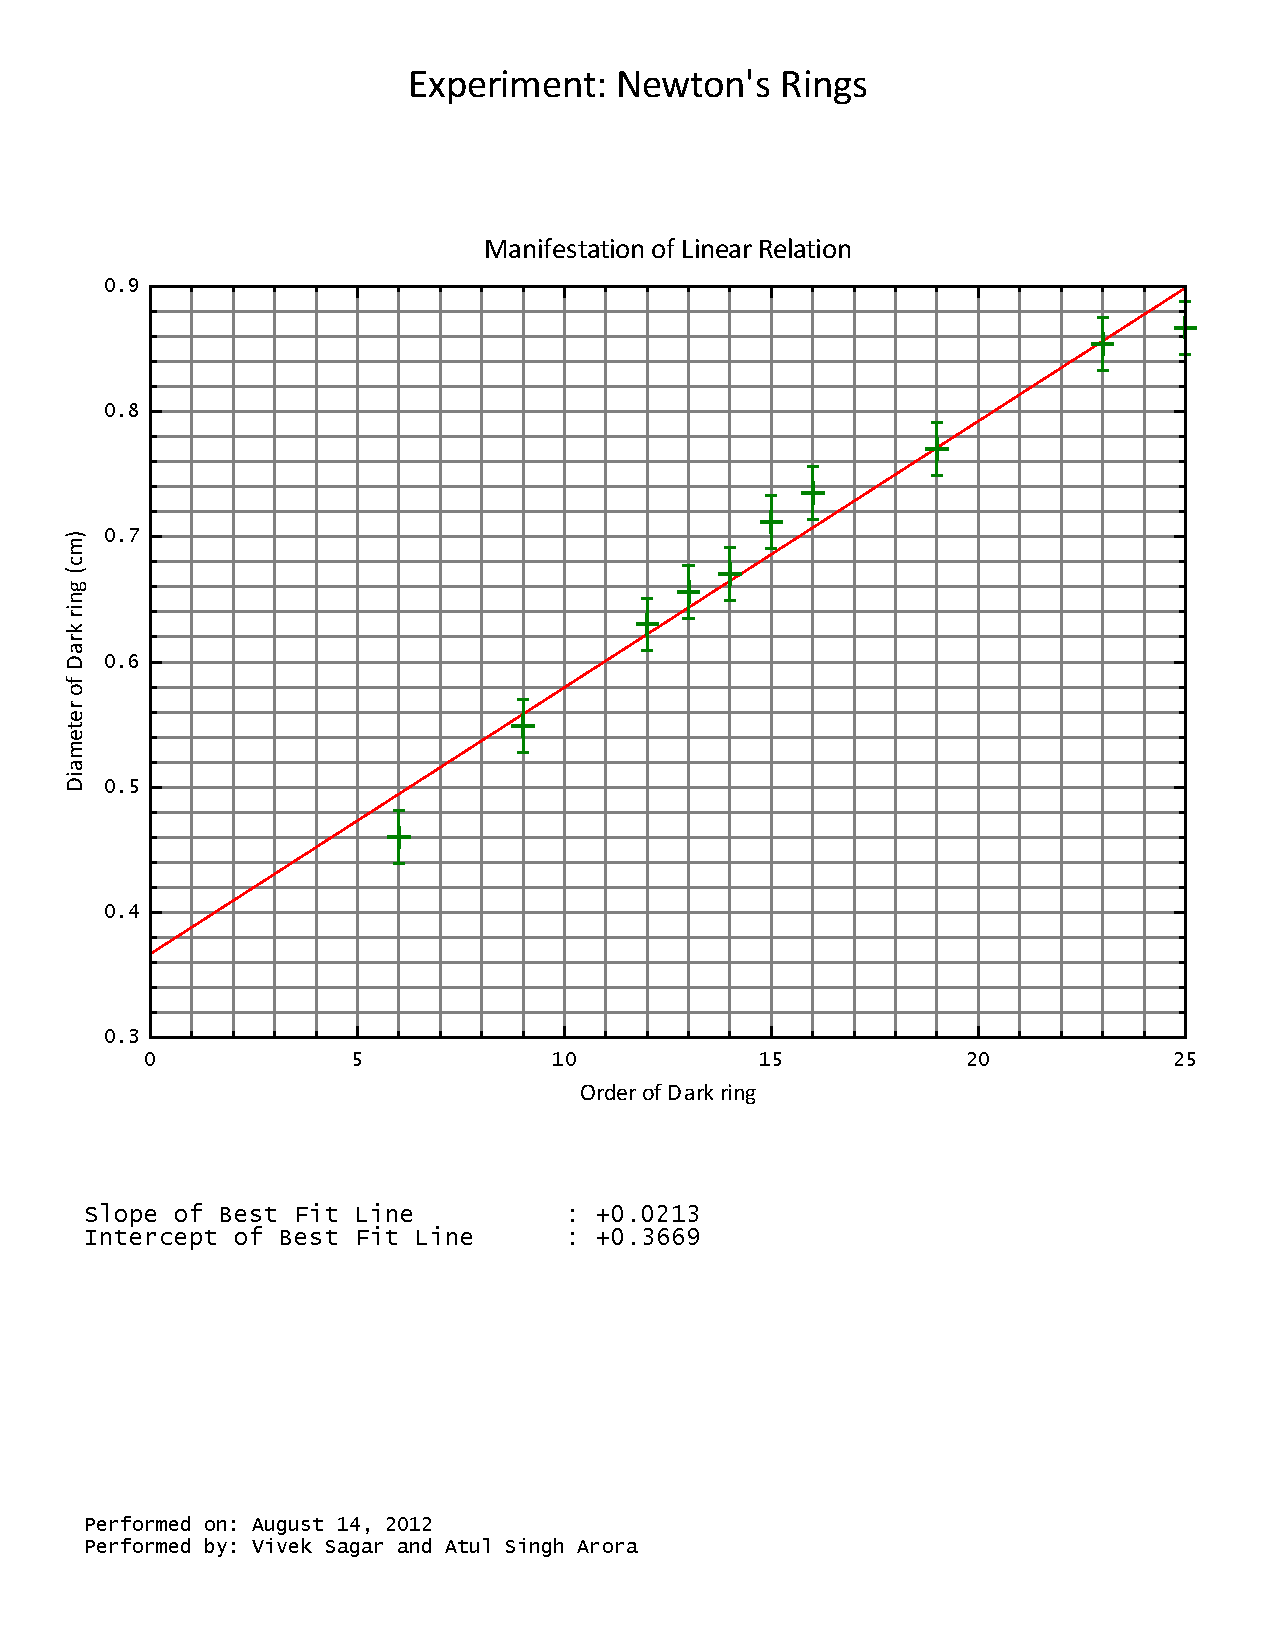
\includegraphics[width=1.3\linewidth]{gfx/1_linear.pdf}
		\end{center}
	\caption[Diameter Squared vs Order of Ring]{Least Square Fit of Diameter Squared vs Order of Ring}
	\label{1_graph}
	\end{figure}

\section{Result}
	The expected wavelength of sodium vapour lamp is $589.5$ nm. \\
	Experimentally, the wavelength, $\lambda$ was found to be \\
	$598.16\pm 3.25\%$ (standard deviation of the slope).\\
	Accuracy error is $1.5\%$, within the precision.
